%----------------------------------------------------------------------------
\chapter{Technologies}

This chapter presents the technologies used to build the deep learning models and create client and server applications.

\section{Deep learning}

I used the Python\cite{Python} programming language in deep learning-related tasks. Python is an interpreted, dynamically typed, high-level language with an object-oriented approach. Numerous libraries offer a deep learning repertoire in Python. However, two libraries stand out from these: PyTorch and TensorFlow. I only describe the technologies I used during this work in the following. My choice was driven primarily by the desire for Android interoperability, which is currently not widely supported by other tools than the selected ones.

\subsection{TensorFlow}

TensorFlow\cite{TensorFlow} is an open-source machine learning platform developed by Google Brains. It provides rich Python and C APIs and works well with the popular Keras neural network library. TF also works well with the Colaboratory environment where GPU/TPU-based works are easy to build without local resources. In 2019, TensorFlow 2.0 was released with Eager mode, which broke up with the former ``define-and-run'' scheme (where a network is statically defined and fixed, and then, the user periodically feeds it with batches of training data). Eager uses a ``define-by-run'' approach\cite{TensorFlowEager}, where operations are immediately evaluated without building graphs.

TensorFlow uses Google's protobuf\cite{Protobuf} format to store models. In this case, a .proto file defines a scheme, and Protocol Buffers generates the content. It is a denser format than XML or JSON, and it supports fast serialization, prevents scheme-violations, and guarantees type-safety\cite{ProtobufVsFlatbuf}. In turn, protobuf files are not as human-readable as opposed to JSON or XML.

TensorFlow Lite is a lightweight, speed, or storage optimized format to deploy models on smartphones and IoT devices. Trained models can be transformed into this format with the TFLite converter. TFLite uses the Flat Buffer\cite{Flatbuf} format. It is similar to TensorFlow's protobuf; the main difference is that Flat Buffers do not require deserializing the entire content (coupled with per-object memory allocation) before accessing an item in it. Therefore, these files consume significantly less memory than protobufs. On the other hand, Flat Buffer encoding is more complicated than in JSON/protobuf formats - for this reason, TensorFlow does not use it. It is also why TFLite models cannot be trained.

During TFLite conversion, it can be selected whether it is required to minimize model size further with a slight model accuracy trade-off or not. These are the quantization options used to achieve further performance gains ($2-3\times$ faster inference, $2-4\times$ smaller networks). I used full integer quantization\cite{TensorFlowQuant} in which all the model maths are int8 based instead of the original float32.

The TensorBoard component provides a helpful visualization tool where users see a dashboard of model performance and training/evaluation details. It can also display the current images fed to the network, the model's answer, and many more. I used this tool to monitor the training/evaluation process.

\subsection{TensorFlow Object Detection API}

TensorFlow's Object Detection API\cite{TensorFlowObjDetAPI} is an open-source framework built on top of TensorFlow to solve complex computer vision tasks, like object detection or semantic segmentation. The library provides a model zoo in which pre-trained models are available. The API supports one-staged meta architectures like SSD, RetinaNet, or CenterNet and two-staged R-CNN variants. However, other types like the YOLO variants are missing.

There are many parameters to tweak during model creation. The API has introduced a configuration language that can fine-tune the training pipeline - e.g., data source, backbone, pre-processing steps, optimization algorithms, and input/output directories. The configuration parameters are described in the corresponding .proto files. The configuration handles architecture level modifications (like different backbone CNNs to use). However, the number of options here is quite limited, customization is cumbersome, and the pipeline is easy to break, which in my opinion, is a big downside.

During this work, support for TF2 has arrived, making it possible to use Keras models in detector architectures. The library has actively evolved in the past years. Although reliability issues often arise, rapid implementations of the latest research (e.g., FPN, CenterNet) helped me understand novel concepts.

\subsection{PyTorch}

PyTorch\cite{PyTorch} is an open-source machine learning framework primarily developed by Meta/Facebook AI Research lab. In the previous years, the community started to use it more extensively, and numerous research implementations were written in it. PyTorch offers a pythonic and object-oriented approach, while TensorFlow has several options to choose from. In my opinion, developing in PyTorch requires more coding than using TensorFlow with Keras. However, it feels more stable and less fragile. The framework also has good interoperability with the Open Neural Network Exchange (ONNX)\cite{ONNX} format, which aims to bridge the compatibility gap between different libraries and frameworks. The PyTorch Mobile module provides both iOS and Android deployment with quantization and optimization. However, it is in the beta stage at the time of this work.

After evaluating the frameworks, I decided to work with TensorFlow/Keras. My primary motivations were finding more documentation for Android, and I assumed it was easier to work with an already matured tool (TensorFlow Lite) than the more risky beta stage PyTorch Mobile.

\subsection{Environment}

The environment in which I worked was Google Colaboratory Pro. I was using Nvidia Tesla V100 SXM2 GPUs with 16 GB memory most of the time. At the beginning of a project, a realm is created or loaded from Google Drive. A realm is where the project saves its checkpoints and training logs. Realms are the sandboxes of notebook instances, making it possible to run them parallel seamlessly. Two types of projects/sessions can be: single training or hyperparameter optimization. For the latter, I used Keras Tuner. An overview of the environment can be seen in Figure \ref{fig:training_environment}.

\begin{figure}[htb]
 \centerline{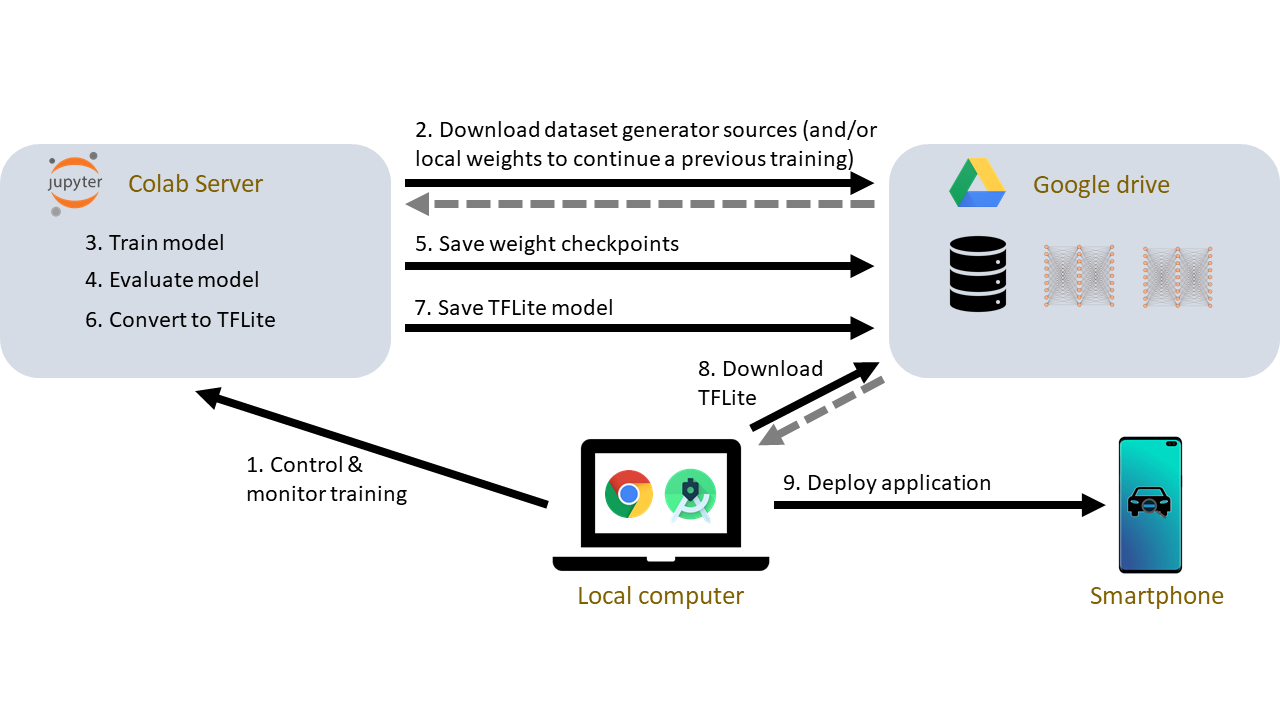
\includegraphics[width=1.0\columnwidth]{.//Figure/Technologies/training_environment.png}}
 \caption{High-level overview of a session in the training environment.}
 \label{fig:training_environment}
\end{figure}

Primarily, I monitored the training on TensorBoard, which shows a dashboard of the running session. After every epoch, the current model is evaluated. On these occasions, model checkpoints are saved (for early stopping and state preservation in case of a failure). After the training process, a standalone evaluation can be executed to verify the results and display the selected loss/protocol metrics.

The model can be saved in three different ways:

\begin{itemize}
  \item First, all the training files and checkpoints are zipped and saved to Google Drive.
  \item Second, only the latest (or the selected) checkpoint is preserved, and detailed log files are discarded (only metrics are retained like loss; model outputs for specific images are dropped) and saved to Drive.
  \item The third option is to convert the model to TFLite and save it.
\end{itemize}

\pagebreak
\section{Application}

I used the Kotlin programming language\cite{Kotlin} for the frontend and the backend. Kotlin is a statically typed, cross-platform language with type inference. In addition to the object-oriented approach, it also contains functional programming tools.

\subsection{Frontend}

Android provides an extensive application development ecosystem. I used the AndroidX namespace elements, which replaced the previous Support Library since Android 9.0. It is part of Android Jetpack, a collection of components for which the platform promises long-term support. The application extensively uses the CameraX API to manage device cameras. The ViewModel component moderates between the user interface and the business logic. The app contains a relational database implemented by the Room Persistence Library, which provides an abstraction layer over SQLite to more robust database access. To boost user experience, I decided to use a text-to-speech engine to read aloud alerts (useful if a user wants notifications while driving or wants to hear how to use tips).

Material Design defines guidelines for building the interface to maximize user experience. On Android, Material elements supported by the platform can be accessed through a library. The application uses its concepts, styles, icons, fonts, and UI elements (e.g., Floating Action Button, Snackbar).

\subsection{Backend}

I used Ktor\cite{Ktor} for the backend. It is an open-source, asynchronous framework for creating microservices and web applications. JSON data handling was implemented with the Gson library. I tested the server API with Postman, and for web scraping, I used ParseHub.

